% !TEX TS-program = pdflatexmk

\documentclass[14pt]{beamer}
\usepackage{newtxtext,newtxmath}
\usepackage{microtype}
\usepackage[english]{babel}
\usepackage{hyperref}
\usepackage{graphicx}
\usepackage{listings}
\lstloadlanguages{Python}
\lstset{language=Python}
\lstset{%
basicstyle=\ttfamily\bfseries,
keywordstyle=\color{blue}, emph={self}, emphstyle={\color{blue}},
identifierstyle=,
commentstyle=\color{brown},
stringstyle=\color{green!50!black},
showstringspaces=false,
emphstyle={[2]\color{purple}},
}
\usepackage{tikz}
\usepackage{pgfplots}
\usepackage{forest}
\usetikzlibrary{calc}
\usetikzlibrary{shapes}
\usetikzlibrary{positioning}
\usetikzlibrary{arrows}
\usepackage{array}
\newcolumntype{L}[1]{>{\raggedright\let\newline\\\arraybackslash\hspace{0pt}}m{#1}}

\mode<presentation>{
\usetheme{Madrid}
\definecolor{uabgreen}{cmyk}{.89,.31,.78,.17}
\usecolortheme[named=uabgreen]{structure}
\setbeamertemplate{navigation symbols}{}
\setbeamertemplate{footline}[frame number]
\setbeamertemplate{section in toc}[square]
\setbeamertemplate{subsection in toc}[square]
\setbeamertemplate{items}[square]
\setbeamercovered{transparent=5}
}

\newcommand{\keyword}[1]{{\color{blue}#1}}
\newcommand{\cmnt}[1]{{\color{gray}#1}}
\newcommand{\str}[1]{{\color{green!50!black}#1}}
\newcommand{\num}[1]{{\color{green!55!blue}#1}}
\newcommand{\defn}[1]{{\color{purple}#1}}

\newcommand{\limpl}{\Rightarrow}
\newcommand{\liff}{\Leftrightarrow}

\newcommand{\tab}{\hspace{1em}}

\author[Dr. Bethard]{Dr. Steven Bethard}
\institute[UAB CIS]{%
Computer and Information Sciences\\
University of Alabama at Birmingham}

\AtBeginSection[]
{
  \begin{frame}<beamer>{Outline}
    \tableofcontents[currentsection]
  \end{frame}
}

\tikzset{
  invisible/.style={opacity=0,text opacity=0},
  text visible on/.code={%
    \alt<#1>{}{\pgfkeysalso{text opacity=0}}
  },
  visible on/.code={%
    \alt<#1>{}{\pgfkeysalso{invisible}}
  },
  filled on/.code={%
    \alt<#1>{\pgfkeysalso{fill=gray}}{}
  },
  alt/.code n args={3}{%
    \alt<#1>{\pgfkeysalso{#2}}{\pgfkeysalso{#3}}
  },
}
\forestset{
  edge weight/.style={
    edge label={node[midway,above,sloped]{#1}}},
  invisible/.style={
    /tikz/invisible,
    edge={/tikz/invisible}},
  visible on filled on/.code n args={2}{%
    \alt<#1>{\alt<#2>{\pgfkeysalso{fill=gray}}{}}{\pgfkeysalso{invisible}}
  },
  visible on/.code={%
    \alt<#1>{}{\pgfkeysalso{invisible}}
  },
}

\newlength{\wumpusgridsize}
\newenvironment{wumpusgrid}[2]{%
\setlength{\wumpusgridsize}{#2}
\begin{tikzpicture}
\draw[very thick,step=\wumpusgridsize] (0,0) grid (#1\wumpusgridsize, #1\wumpusgridsize);
}{%
\end{tikzpicture}
}
\newcommand{\wumpustop}[5][]{%
\only<#2>{\node[#1] at (#3\wumpusgridsize+0.5\wumpusgridsize,#4\wumpusgridsize+0.75\wumpusgridsize) {#5};}
}
\newcommand{\wumpusbottom}[5][]{%
\only<#2>{\node[#1] at (#3\wumpusgridsize+0.5\wumpusgridsize,#4\wumpusgridsize+0.25\wumpusgridsize) {#5};}
}
\newcommand{\wumpusagent}[3]{\wumpusbottom{#1}{#2}{#3}{\fbox{A}}}
\newcommand{\wumpuspercept}[4]{%
\only<#1>{\node[red,inner sep=0pt] at (#2\wumpusgridsize+0.25\wumpusgridsize,#3\wumpusgridsize+0.75\wumpusgridsize) {\textbf{#4}};}
}
\newcommand{\wumpusknowledge}[4]{%
\only<#1>{\node[draw,cloud,inner sep=0pt,text width=1em,align=center] at (#2\wumpusgridsize+0.75\wumpusgridsize,#3\wumpusgridsize+0.75\wumpusgridsize) {\footnotesize #4};}
}

\usepackage{relsize}

\title{Probabilistic Reasoning}
\date{13 Mar 2014}

\newcommand{\alertit}[1]{\alert{\textit{#1}}}

\newcommand{\scriptfactor}[2]{%
\mbox{\scriptsize\setlength{\arraycolsep}{0.2em}$\left(
\begin{array}{ #1 l }
#2
\end{array}
\right)$}
}

\tikzset{
  bn variable/.style={draw,ellipse,inner sep=0.2em},
  bn depends on/.style={draw,triangle 45-,thick},
  bn table/.style={draw,inner sep=0em,font=\small},
}

\newcommand{\rainbayesnet}[1]{
\setlength{\tabcolsep}{0.2em}
\begin{tikzpicture}[font=#1]
\node[bn variable] at (.5\textwidth, .65\textheight) (C) {Cloudy};
\node[bn table,above=0.2em of C] {#1
\begin{tabular}{ c }
\textbf{P(C)} \\
\hline
.50
\end{tabular}
};
\node[bn variable] at (0.35\textwidth, .5\textheight) (S) {Sprinkler};
\node[bn table,left=0.2em of S] {#1
\begin{tabular}{ c c }
\textbf{C} & \textbf{P(S|C)} \\
\hline
T & .10 \\
F & .50
\end{tabular}
};
\node[bn variable] at (0.65\textwidth, .5\textheight) (R) {Rain};
\node[bn table,right=0.2em of R] {#1
\begin{tabular}{ c c }
\textbf{C} & \textbf{P(R|C)} \\
\hline
T & .80 \\
F & .20
\end{tabular}
};
\node[bn variable] at (.5\textwidth, .35\textheight) (W) {Wet Grass};
\node[bn table,below=0.2em of W] {#1
\begin{tabular}{ c c c }
\textbf{S} & \textbf{R} & \textbf{P(W|S,R)} \\
\hline
T & T & .99 \\
T & F & .90 \\
F & T & .90 \\
F & F & .00
\end{tabular}
};
\path[bn depends on] (S) -- (C);
\path[bn depends on] (R) -- (C);
\path[bn depends on] (W) -- (S);
\path[bn depends on] (W) -- (R);
\end{tikzpicture}
}

\begin{document}

\begin{frame}
\titlepage
\end{frame}

\begin{frame}{Outline}
\tableofcontents
\end{frame}

\section{Bayesian Networks}

\subsection{Bayesian Network Basics}

\begin{frame}[label=bayes-net-definition]{Bayesian Networks}
\begin{block}{Definition}
A \alert{Bayesian Network} is a data structure for representing independence relations among random variables
\end{block}
\begin{center}
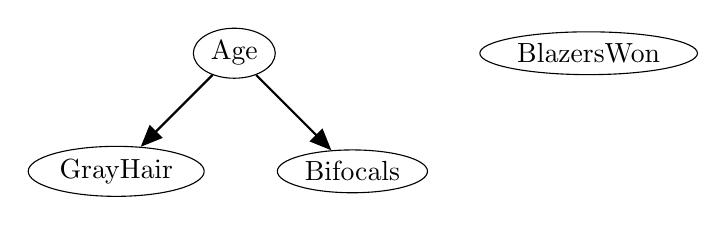
\begin{tikzpicture}
\node[bn variable] at (1.5, 1.5) (A) {Age};
\node[bn variable] at (0, 0) (GH) {GrayHair};
\node[bn variable] at (3, 0) (B) {Bifocals};
\node[bn variable] at (6, 1.5) (BW) {BlazersWon};
\path[bn depends on] (GH) -- (A);
\path[bn depends on] (B) -- (A);
\end{tikzpicture}
\end{center}
\pause
$
\begin{array}{ll}
\lefteqn{P(\textit{Age}, \textit{GrayHair}, \textit{Bifocals}, \textit{BlazersWon}) = \mbox{}}\\ 
& P(\textit{Age}, \textit{GrayHair}, \textit{Bifocals})P(\textit{BlazersWon})
\end{array}
$
\pause
\smallskip
$
\begin{array}{ll}
\lefteqn{P(\textit{GrayHair},\textit{Bifocals}|\textit{Age}) = \mbox{}}\\ 
& P(\textit{GrayHair}|\textit{Age})P(\textit{Bifocals}|\textit{Age})
\end{array}
$ \\
\end{frame}

\begin{frame}{Bayesian Networks}
	\begin{block}{Components}
		\begin{itemize}
			\item Random variables (nodes)
			\item Directed links from \textit{parent} nodes to \textit{child} nodes
			\item $\mathbf{P}(X_{i}|\textit{Parents}(X_{i}))$ tables for each node
			\item Links form no cycles
		\end{itemize}
	\end{block}
	\pause
	\begin{block}{Intuitions}
		\begin{itemize}
			\item Links indicate \emph{direct} influence
			\item Causes usually near top
			\item Effects usually near bottom
		\end{itemize}
	\end{block}
\end{frame}

\begin{frame}[label=bayes-net-full-example]{Full Bayesian Network Example}
\begin{center}
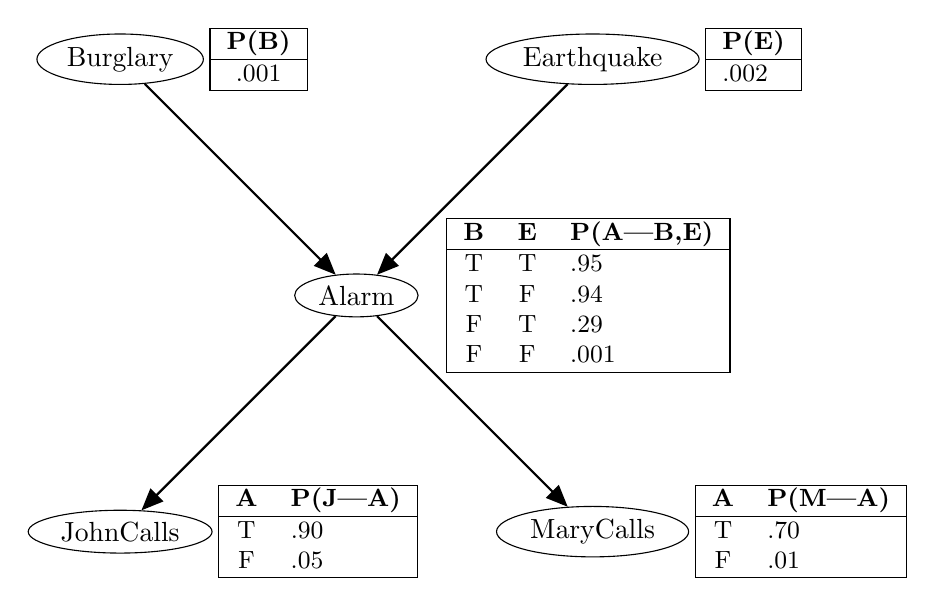
\begin{tikzpicture}
\node[bn variable] at (0, 6) (B) {Burglary};
\node[bn table,right=0.2em of B] {
\begin{tabular}{ c }
\textbf{P(B)} \\
\hline
.001
\end{tabular}
};
\node[bn variable] at (6, 6) (E) {Earthquake};
\node[bn table,right=0.2em of E] {
\begin{tabular}{l}
\textbf{P(E)} \\
\hline
.002
\end{tabular}
};
\node[bn variable] at (3, 3) (A) {Alarm};
\node[bn table,right=1em of A] {
\begin{tabular}{ c c l }
\textbf{B} & \textbf{E} & \textbf{P(A|B,E)} \\
\hline
T & T & .95 \\
T & F & .94 \\
F & T & .29 \\
F & F & .001
\end{tabular}
};
\node[bn variable] at (0, 0) (J) {JohnCalls};
\node[bn table,right=0.2em of J] {
\begin{tabular}{ c l }
\textbf{A} & \textbf{P(J|A)} \\
\hline
T & .90 \\
F & .05
\end{tabular}
};
\node[bn variable] at (6, 0) (M) {MaryCalls};
\node[bn table,right=0.2em of M] {
\begin{tabular}{ c l }
\textbf{A} & \textbf{P(M|A)} \\
\hline
T & .70 \\
F & .01
\end{tabular}
};
\path[bn depends on] (A) -- (B);
\path[bn depends on] (A) -- (E);
\path[bn depends on] (J) -- (A);
\path[bn depends on] (M) -- (A);
\end{tikzpicture}
\end{center}
\end{frame}

\subsection{The Full Joint Distribution}
\begin{frame}{Representing the Full Joint Distribution}
	\begin{block}{Key Formula}
		$P(x_{1},\ldots,x_{n}) = \prod\limits_{i=1}^{n}{P(x_{i}|\textit{parents}(X_{i}))}$
	\end{block}
	\begin{block}{Example}
		$
		\begin{array}{lll}
			\lefteqn{P(j, m, a, \lnot b, \lnot e)}
			\\
			& = & \pause
			      P(j|\textit{parents}(j)) \cdot
			      P(m|\textit{parents}(m)) \cdot
			      \ldots
			\\
			& = & \pause
			      P(j|a) \cdot
			      P(m|a) \cdot
			      P(a|\lnot b, \lnot e) \cdot
			      P(\lnot b) \cdot
			      P(\lnot e)
			\\
			& = & \pause
			      0.90 \cdot
			      0.70 \cdot
			      0.001 \cdot
			      0.999 \cdot
			      0.998
			\\
			& = & \pause
			      0.00062
		\end{array}
		$
	\end{block}
\end{frame}
\begin{frame}{A Simple Inference Algorithm}
	\begin{block}{Goal: Answer Queries}
		\begin{itemize}
			\item One query variable given some evidence
			\item $\mathbf{P}(X|y_{1},\ldots,y_{n})$
		\end{itemize}
	\end{block}
	\pause
	\begin{block}{Solution: Enumeration}
		$
		\begin{array}{@{}lll@{}}
			\lefteqn{\mathbf{P}(X|y_{1},\ldots,y_{n})} \\
			& = & \alpha\mathbf{P}(X,y_{1},\ldots,y_{n}) \\
			& = & \alpha\sum\limits_{z_{1},\ldots,z_{k} \in \mathbf{\overline{XY}}}
			      {\mathbf{P}(X,y_{1},\ldots,y_{n},z_{1},\ldots,z_{k})} \\
			& = & \alpha\sum\limits_{z_{1},\ldots,z_{k} \in \mathbf{\overline{XY}}}
			      {\mathbf{P}(X|\ldots)
			       P(y_{1}|\ldots)
			       \ldots
			       P(z_{k}|\ldots)} \\
		\end{array}
		$
	\end{block}
\end{frame}

\begin{frame}[label=enumeration-worst-case]{Enumeration Worst Case}
\begin{block}{Enumeration Formula}
$
\mathbf{P}(X|y_{1},\ldots,y_{n}) = 
\alpha\sum\limits_{z_{1},\ldots,z_{k} \in \mathbf{\overline{XY}}}
          {\mathbf{P}(X|\mbox{\scriptsize\ldots})
           P(y_{1}|\mbox{\scriptsize\ldots})
           \ldots
           P(z_{k}|\mbox{\scriptsize\ldots})}
$
\end{block}
\pause
\begin{columns}
\begin{column}{1.5in}
\begin{center}
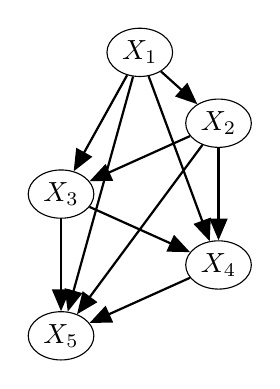
\begin{tikzpicture}
\node[bn variable] at (1, 3.6) (1) {$X_1$};
\node[bn variable] at (2, 2.7) (2) {$X_2$}
  edge[bn depends on] (1);
\node[bn variable] at (0, 1.8) (3) {$X_3$}
  edge[bn depends on] (1)
  edge[bn depends on] (2);
\node[bn variable] at (2, .9) (4) {$X_4$}
  edge[bn depends on] (1)
  edge[bn depends on] (2)
  edge[bn depends on] (3);
\node[bn variable] at (0, 0) (5) {$X_5$}
  edge[bn depends on] (1)
  edge[bn depends on] (2)
  edge[bn depends on] (3)
  edge[bn depends on] (4);
\end{tikzpicture}
\smallskip
Query: $P(X_{5})$
\end{center}
\end{column}
\pause
\begin{column}{2.5in}
\begin{block}{Worst Case in General}
\begin{itemize}
\item $\approx n$ parents per node
\item $\approx n$ variables not in query
\item $d$ values per variable
\end{itemize}
Time Complexity: \pause $O(nd^{n})$
\end{block}
\end{column}
\end{columns}
\end{frame}

\subsection{Constructing Bayesian Networks}

\begin{frame}[label=constructing-networks]{Avoiding Fully Connected Networks}
\begin{block}{Principles}
\begin{enumerate}
\item Add root causes
\item\label{add-leaf-effects} Add variables directly influenced by leaves
\item If variables left, goto \ref{add-leaf-effects}
\end{enumerate}
\end{block}
\medskip
\begin{columns}[T]
\begin{column}{2.2in}
\uncover<2->{
Good: \\
\footnotesize \textit{Age}, \textit{GrayHair}, \textit{Bifocals}, \textit{ReadDist}} \\
\centering
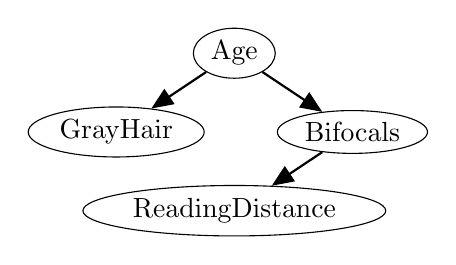
\begin{tikzpicture}
\node[bn variable,visible on={3-}] at (1.5, 2) (A) {Age};
\node[bn variable,visible on={4-}] at (0, 1) (G) {GrayHair}
  edge[bn depends on, visible on={5-}] (A);
\node[bn variable,visible on={6-}] at (3, 1) (B) {Bifocals}
  edge[bn depends on, visible on={7-}] (A);
\node[bn variable,visible on={8-}] at (1.5, 0) (R) {ReadingDistance}
  edge[bn depends on, visible on={9-}] (B);
\end{tikzpicture}
\end{column}
\begin{column}{2.2in}
\uncover<10->{
Bad: \\
\footnotesize \textit{ReadDist}, \textit{GrayHair}, \textit{Bifocals}, \textit{Age}} \\
\centering
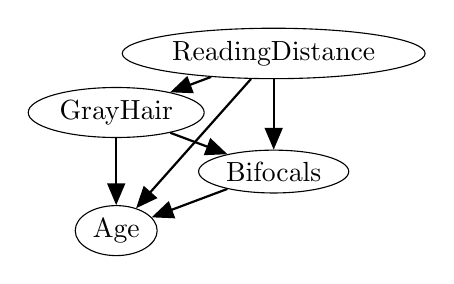
\begin{tikzpicture}
\node[bn variable,visible on={11-}] at (2, 2.25) (R) {ReadingDistance};
\node[bn variable,visible on={12-}] at (0, 1.5) (G) {GrayHair}
  edge[bn depends on, visible on={13-}] (R);
\node[bn variable,visible on={14-}] at (2, 0.75) (B) {Bifocals}
  edge[bn depends on, visible on={15-}] (R)
  edge[bn depends on, visible on={15-}] (G);
\node[bn variable,visible on={16-}] at (0, 0) (A) {Age}
  edge[bn depends on, visible on={17-}] (R)
  edge[bn depends on, visible on={17-}] (G)
  edge[bn depends on, visible on={17-}] (B);
\end{tikzpicture}
\end{column}
\end{columns}
\end{frame}

\begin{frame}{Bayesian Network Exercise}
	\begin{block}{Construct a Network}
		\begin{itemize}
			\item The fire alarm usually goes off when there's a fire
			\item When the alarm rings everyone usually exits together
			\item Most of the time there's smoke when there's a fire
			\item Someone sometimes pulls the fire alarm ``as a joke''
			\item The fire trucks usually come when the alarm goes off
			\item Sometimes everyone exits together for a picnic
		\end{itemize}
	\end{block}
\end{frame}

\begin{frame}[label=network-exercise-solution]{Bayesian Network Exercise}
One possible solution:
\begin{center}
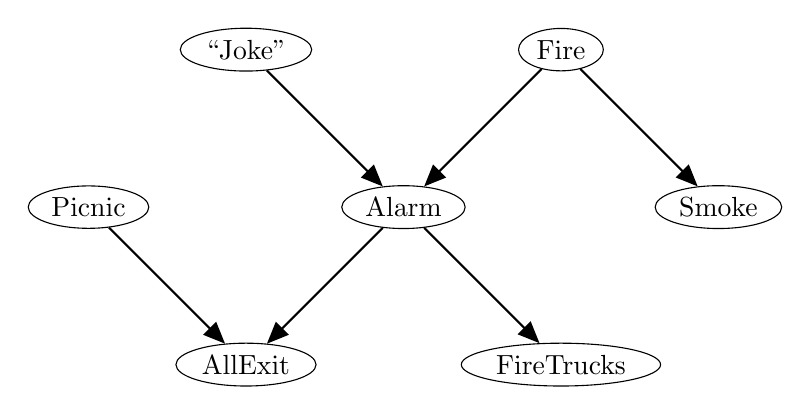
\begin{tikzpicture}
\node[bn variable] at (2, 4) (J) {``Joke''};
\node[bn variable] at (6, 4) (F) {Fire};
\node[bn variable] at (0, 2) (P) {Picnic};
\node[bn variable] at (4, 2) (A) {Alarm}
  edge[bn depends on] (J)
  edge[bn depends on] (F);
\node[bn variable] at (8, 2) (S) {Smoke}
  edge[bn depends on] (F);
\node[bn variable] at (2, 0) (AE) {AllExit}
  edge[bn depends on] (P)
  edge[bn depends on] (A);
\node[bn variable] at (6, 0) (FT) {FireTrucks}
  edge[bn depends on] (A);
\end{tikzpicture}
\end{center}
\end{frame}

\section{Efficient Exact Inference}

\subsection{Enumeration}

\begin{frame}{Drawbacks of Simple Enumeration}
\begin{block}{Recall: Simple Enumeration}
Time Complexity: $O(nd^{n})$
\end{block}
\pause
\begin{block}{Example}
{\small$\begin{array}{@{}lll@{}}
P(b|j,m) & = & \alpha\sum\limits_{e'}\sum\limits_{a'}P(b)P(e')P(a'|b,e')P(j|a')P(m|a') \\
         & = & \alpha(P(b)P(e)P(a|b,e)P(j|a)P(m|a) + \mbox{}\\
         &   &   \tab P(b)P(e)P(\lnot a|b,e)P(j|\lnot a)P(m|\lnot a) + \mbox{}\\
         &   &   \tab P(b)P(\lnot e)P(a|b,\lnot e)P(j|a)P(m|a) + \mbox{}\\
         &   &   \tab P(b)P(\lnot e)P(\lnot a|b,\lnot e)P(j|\lnot a)P(m|\lnot a))
\end{array}$}
\\
\medskip
\pause Problem: \pause We calculate $P(b)$, $P(e)$ and $P(\lnot e)$ many times!
\end{block}
\end{frame}

\begin{frame}{More Intelligent Summation}
\begin{block}{Moving Terms in Algebra}
$
\begin{array}{lll}
\lefteqn{abd + abe + acf + acg} \\
& = & \pause a(bd + be + cf + cg) \\
& = & \pause a(b(d + e) + c(f + g)) \\
\end{array}
$
\end{block}
\pause
\begin{block}{Moving Terms in Bayesian Network Calculations}
{\small$\begin{array}{lll}
P(b|j,m) & = & \alpha\sum\limits_{e'}\sum\limits_{a'}P(b)P(e')P(a'|b,e')P(j|a')P(m|a') \\
& = & \pause
\alpha P(b)\sum\limits_{e'}\sum\limits_{a'}P(e')P(a'|b,e')P(j|a')P(m|a') \\
& = & \pause
\alpha P(b)\sum\limits_{e'}P(e')\sum\limits_{a'}P(a'|b,e')P(j|a')P(m|a')
\end{array}$}
\end{block}
\end{frame}

\begin{frame}[label=depth-first-calculation]{Calculations through Depth First Search}
\centering
$P(b|j,m) = \alpha P(b)\sum\limits_{e'}P(e')\sum\limits_{a'}P(a'|b,e')P(j|a')P(m|a')$ \\
\bigskip
\small
\begin{forest}
[{$P(b)$}
  [{$P(e)$}
    [{$P(a|b,e)$}
      [{$P(j|a)$}
        [{$P(m|a)$}]
      ]
    ]
    [{$P(\lnot a|b,e)$}
      [{$P(j|\lnot a)$}
        [{$P(m|\lnot a)$}]
      ]
    ]
  ]
  [{$P(\lnot e)$}
    [{$P(a|b,\lnot e)$}
      [{$P(j|a)$}
        [{$P(m|a)$}]
      ]
    ]
    [{$P(\lnot a|b,\lnot e)$}
      [{$P(j|\lnot a)$}
        [{$P(m|\lnot a)$}]
      ]
    ]
  ]
]
\end{forest}
\end{frame}

\subsection{Factors}

\begin{frame}[label=factors]{Factors}
\setbeamercovered{invisible}
Avoid duplicate calculations by using \alert{factors}, which store:
\begin{itemize}
\item A set of variables
\item A number for each possible assignment of values
\end{itemize}
\pause
\begin{center}
\setlength{\arraycolsep}{0.2em}
\small
$\begin{array}{ l l l l }
P(m|A)
& = f(A)
& = \left(\begin{array}{ r c l }
a & \rightarrow & 0.70 \\
\lnot a & \rightarrow & 0.01
\end{array}\right)
\\[1em]
\pause
P(A|B,E)
& = g(A,B,E)
& = \left(\begin{array}{ r r r c l }
a & b & e & \rightarrow & 0.95 \\
a & b & \lnot e & \rightarrow & 0.94 \\
a & \lnot b & e & \rightarrow & 0.29 \\
a & \lnot b & \lnot e & \rightarrow & 0.001 \\
\lnot a & b & e & \rightarrow & 0.05 \\
\lnot a & b & \lnot e & \rightarrow & 0.06 \\
\lnot a & \lnot b & e & \rightarrow & 0.71 \\
\lnot a & b & \lnot e & \rightarrow & 0.999
\end{array}\right)
\end{array}$
\end{center}
\end{frame}

\begin{frame}{Factor Product}
\setbeamercovered{invisible}
The \alert{factor product} of factors $f$ and $g$ yields a factor with:
\begin{itemize}
\item The union of the variables of $f$ and $g$
\item Values that are the product of the corresponding rows
\end{itemize}
\medskip
\uncover<2->{
{\small\setlength{\arraycolsep}{0.2em}\[
\left(\begin{array}{ r r c l }
j & a & \rightarrow & 0.90 \\
j & \lnot a & \rightarrow & 0.05 \\
\lnot j & a & \rightarrow & 0.10 \\
\lnot j & \lnot a & \rightarrow & 0.95
\end{array}\right)
\times
\left(\begin{array}{ r r c l }
m & a & \rightarrow & 0.70 \\
m & \lnot a & \rightarrow & 0.01 \\
\lnot m & a & \rightarrow & 0.30 \\
\lnot m & \lnot a & \rightarrow & 0.99
\end{array}\right)
= 
\uncover<3->{
\left(\begin{array}{ r r r c l }
j & m & a & \rightarrow & \uncover<4->{0.63} \\
j & m & \lnot a & \rightarrow & \uncover<5->{0.0005} \\
j & \lnot m & a & \rightarrow & \uncover<6->{0.27} \\
j & \lnot m & \lnot a & \rightarrow & \uncover<7->{0.0495} \\
\lnot j & m & a & \rightarrow & \uncover<8->{0.07} \\
\lnot j & m & \lnot a & \rightarrow & \uncover<8->{0.0095} \\
\lnot j & \lnot m & a & \rightarrow & \uncover<8->{0.03} \\
\lnot j & \lnot m & \lnot a & \rightarrow & \uncover<8->{0.9405} \\
\end{array}\right)
}
\]}
}
\end{frame}

\begin{frame}{Factor Marginalization}
The \alert{factor marginalization} of factor $f$ for variable $A$ yields a factor with:
\begin{itemize}
\item The variables of $f$, minus the variable $A$
\item Values that are the sum of the corresponding rows
\end{itemize}
\medskip
\uncover<2->{
{\small\setlength{\arraycolsep}{0.2em}
\[
\mathlarger{\sum}_{A}
\left(\begin{array}{ @{} r r r c l @{} }
j & m & a & \rightarrow & 0.63 \\
j & m & \lnot a & \rightarrow & 0.0005 \\
j & \lnot m & a & \rightarrow & 0.27 \\
j & \lnot m & \lnot a & \rightarrow & 0.0495 \\
\lnot j & m & a & \rightarrow & 0.07 \\
\lnot j & m & \lnot a & \rightarrow & 0.0095 \\
\lnot j & \lnot m & a & \rightarrow & 0.03 \\
\lnot j & \lnot m & \lnot a & \rightarrow & 0.9405 \\
\end{array}\right)
=
\uncover<3->{
\left(\begin{array}{ @{} r r c l @{} }
j & m & \rightarrow & \uncover<4->{0.6305} \\
j & \lnot m & \rightarrow & \uncover<5->{0.3195} \\
\lnot j & m & \rightarrow & \uncover<6->{0.0795} \\
\lnot j & \lnot m & \rightarrow & \uncover<7->{0.9705} \\
\end{array}\right)
}
\]}
}
\end{frame}

\begin{frame}[label=factor-inference]{Exact Inference via Factors}
\small
\setlength{\arraycolsep}{0.2em}
$
\begin{array}{ @{} l @{} l l l @{} }
\lefteqn{P(B|j,m)}
\\
& & = & \displaystyle \alpha P(B)\sum_{e' \in E} P(e') \sum_{a' \in A} P(a'|B,e')P(j|a')P(m|a')
\\
\parbox[c][0.3\textheight]{0em}{} &
\only<2>{
& = & \displaystyle 
\alpha
\scriptfactor{ r }{
b & .001 \\
\lnot b & .999}
\times
\sum_E
\scriptfactor{ r }{
e & .002 \\
\lnot e & .998}
\times
\sum_A
\scriptfactor{ r r r }{
a & b & e & .95 \\
a & b & \lnot e & .94 \\
a & \lnot b & e & .29 \\
a & \lnot b & \lnot e & .001 \\
\lnot a & b & e & .05 \\
\lnot a & b & \lnot e & .06 \\
\lnot a & \lnot b & e & .71 \\
\lnot a & \lnot b & \lnot e & .999}
\times
\scriptfactor{ r }{
a & .9 \\
\lnot a & .05}
\times
\scriptfactor{ r }{
a & .7 \\
\lnot a & .01}
}
\only<3>{
& = & \displaystyle
\alpha
\scriptfactor{ r }{
b & .001 \\
\lnot b & .999}
\times
\sum_E
\scriptfactor{ r }{
e & .002 \\
\lnot e & .998}
\times
\sum_A
\scriptfactor{ r r r }{
a & b & e & .95 \\
a & b & \lnot e & .94 \\
a & \lnot b & e & .29 \\
a & \lnot b & \lnot e & .001 \\
\lnot a & b & e & .05 \\
\lnot a & b & \lnot e & .06 \\
\lnot a & \lnot b & e & .71 \\
\lnot a & \lnot b & \lnot e & .999}
\times
\scriptfactor{ r }{
a & .63 \\
\lnot a & .0005}
}
\only<4>{
& = & \displaystyle
\alpha
\scriptfactor{ r }{
b & .001 \\
\lnot b & .999}
\times
\sum_E
\scriptfactor{ r }{
e & .002 \\
\lnot e & .998}
\times
\sum_A
\scriptfactor{ r r r }{
a & b & e & .5985 \\
a & b & \lnot e & .5922 \\
a & \lnot b & e & .1827 \\
a & \lnot b & \lnot e & .00063 \\
\lnot a & b & e & .000025 \\
\lnot a & b & \lnot e & .00003 \\
\lnot a & \lnot b & e & .000355 \\
\lnot a & \lnot b & \lnot e & .0004995}
}
\only<5>{
& = & \displaystyle
\alpha
\scriptfactor{ r }{
b & .001 \\
\lnot b & .999}
\times
\sum_E
\scriptfactor{ r }{
e & .002 \\
\lnot e & .998}
\times
\scriptfactor{ r r }{
b & e & .598525 \\
b & \lnot e & .59223 \\
\lnot b & e & .183055 \\
\lnot b & \lnot e & .0011295}
}
\only<6>{
& = & \displaystyle
\alpha
\scriptfactor{ r }{
b & .001 \\
\lnot b & .999}
\times
\sum_E
\scriptfactor{ r r }{
b & e & .00119705 \\
b & \lnot e & .59104554 \\
\lnot b & e & .00036611 \\
\lnot b & \lnot e & .001127241}
}
\only<7>{
& = & \displaystyle
\alpha
\scriptfactor{ r }{
b & .001 \\
\lnot b & .999}
\times
\scriptfactor{ r r }{
b & .59224259 \\
\lnot b & .001493351}
}
\only<8>{
& = & \displaystyle
\alpha
\scriptfactor{ r }{
b & .00059224259 \\
\lnot b & .001491857649}
}
\only<9>{
& \approx & \displaystyle
\scriptfactor{ r }{
b & .284 \\
\lnot b & .716}
}
\end{array}
$
\end{frame}

\subsection{Properties}

\begin{frame}{Exact Inference Properties}
Given a network with:
\begin{itemize}
\item $v$ variables
\item $k$ values per variable
\item $p$ parents per variable
\item $r$ rows in the conditional probability tables
\end{itemize}
Worst case time and space complexity:
\begin{description}[Multiply connected]
\item[Singly connected]
$O(r)$ \\
\pause
If $p$ constant-bounded $\Rightarrow$ $O(v)$
\pause
\item[Multiply connected]
$O(k^{v})$ \\
\pause
Cluster variables into tree $\Rightarrow$ $O(r')$
\end{description}
\end{frame}


\section{Approximate Inference}
\begin{frame}[fragile]{Approximate Inference}
Given query $P(X=x|Y_1=z_1,\ldots,Y_n=z_n)$:
\begin{itemize}
\item Generate $k$ assignments of all variables in network
\item Drop assignments inconsistent with {\small$Y_1=z_1,\ldots,Y_n=z_n$}
\item Count assignments where $X\!=\!x$, and divide by $k$
\end{itemize}
\pause
\begin{semiverbatim}\scriptsize\bfseries
\keyword{def} \defn{prior_sample}(bayes_net):
    \pause\cmnt{# generate a value for each variable in the network}
    \cmnt{# variables are sorted from parents to children}
    sample = []
    \keyword{for} node \keyword{in} bayes_net:
        \pause\cmnt{# find the values assigned to the parents}
        parent_samples = [sample[p.index] \keyword{for} p \keyword{in} node.parents]
        \pause\cmnt{# find the probability for this assignment from the table}
        prob = node.get_prob(\keyword{True}, *parent_samples)
        \pause\cmnt{# add True or False according to the distribution}
        sample.append(random.random() < prob)
    \pause\cmnt{# return the complete sample}
    \keyword{return} sample
\end{semiverbatim}
\end{frame}


\subsection{Rejection Sampling}


\begin{frame}[fragile]{Rejection Sampling}
\setbeamercovered{invisible}
	\begin{block}{Key Idea}
		Throw away samples inconsistent with the evidence
	\end{block}
	\medskip
	\pause
	\begin{tabular}{ll}
		Variables: & \textit{Cloudy}, \textit{Sprinkler}, \textit{Rain}, \textit{WetGrass} \\
		Query:     & $P(\textit{Rain}|\textit{Sprinkler}\!=\!\textit{true})$
	\end{tabular}
	\\
	\medskip
	$
	\begin{array}{llll|cc}
		\textit{Cloudy} & \textit{Sprinkler} & \textit{Rain}  & \textit{WetGrass} & \textit{rain} & \lnot\textit{rain} \\
		\hline
		\pause
		\textit{false}  & \textit{false}     & \textit{false} & \textit{false}    &           &            \\
		\pause
		\textit{true}   & \textit{true}      & \textit{false} & \textit{true}     &           & \pause 1   \\
		\pause
		\textit{true}   & \textit{false}     & \textit{false} & \textit{false}    &           &            \\
		\pause
		\textit{false}  & \textit{true}      & \textit{true}  & \textit{true}     & \pause 1  &            \\
		\pause
		\textit{false}  & \textit{true}      & \textit{false} & \textit{true}     &           & \pause 1
	\end{array}
	$
	\\
	\medskip
	\pause
	\tab$P(\textit{Rain}\!=\!\textit{true}|\textit{Sprinkler}\!=\!\textit{true})=\pause\frac{1}{1 + 1 + 1}=\frac{1}{3}$
\end{frame}

\begin{frame}[fragile]{Rejection Sampling Code}
	\begin{semiverbatim}\scriptsize\bfseries
		\keyword{def} \defn{rejection_sampling}(query_var, evidence, bayes_net, samples):
		    \pause\cmnt{# generate a bunch of samples, counting query values}
		    counts = \{\keyword{False}: \num{0}, \keyword{True}: \num{0}\}
		    \keyword{for} _ \keyword{in} range(samples):
		        sample = prior_sample(bayes_net)
		        \pause\cmnt{# if the sample is consistent with the evidence, count it}
		        \keyword{if} all(sample[v.index] == evidence[v] \keyword{for} v \keyword{in} evidence):
		            counts[sample[query_var.index]] += \num{1}
		    \pause\cmnt{# normalize the counts and return the probabilities}
		    \keyword{return} normalize(counts)
		\pause
		\keyword{def} \defn{normalize}(counts):
		    \pause\cmnt{# divide all counts by the total}
		    total = sum(counts.values())
		    \keyword{for} value \keyword{in} counts:
		        counts[value] /= total
		    \pause\cmnt{# return the probabilities}
		    \keyword{return} counts
	\end{semiverbatim}
\end{frame}

\begin{frame}{Rejection Sampling Exercise}
\setbeamercovered{invisible}
\begin{columns}
\begin{column}{0.62\textwidth}
\rainbayesnet{\footnotesize}
\end{column}
\begin{column}{0.35\textwidth}
\small
Calculate: \\
\smallskip
\begin{tabular}{l@{}}
$P(\textit{rain}|\textit{sprinkler})$ \\
5 samples \\
\textit{true} if below random
\end{tabular} \\
\medskip
Random numbers: \\
\smallskip
$
\begin{array}{llll}
\parbox{.22in}{C} & \parbox{.22in}{S}            & \parbox{.22in}{R}             & W                \\
\hline
\alt<2->{F}{0.6}  & \alert<8->{\alt<3->{T}{0.4}} & \alt<4->{F}{0.3}              & \alt<5->{T}{0.8} \\
\alt<6->{F}{0.7}  & \alert<8->{\alt<6->{T}{0.3}} & \alt<6->{F}{0.8}              & \alt<6->{T}{0.6} \\
\alt<6->{T}{0.3}  &            \alt<6->{F}{0.2}  & \alt<6->{T}{0.7}              & \alt<6->{T}{0.3}  \\
\alt<6->{F}{0.9}  & \alert<8->{\alt<6->{T}{0.2}} & \alt<6->{F}{0.4}              & \alt<6->{T}{0.1} \\
\alt<6->{F}{0.8}  & \alert<8->{\alt<6->{T}{0.4}} & \alert<9->{\alt<6->{T}{0.1}}  & \alt<6->{T}{0.9} \\
\end{array}
$ \\
\medskip
\uncover<7->{$P(\textit{rain}|\textit{sprinkler}) = \uncover<10->{\frac{1}{4}}$}
\end{column}
\end{columns}
\end{frame}

\begin{frame}{Rejection Sampling}
	\begin{block}{Properties}
		Given $n$ variables, at most $d$ parents each, $s$ samples drawn and $u$ samples used:
		\begin{itemize}
			\item Time Complexity: \pause $O(nds)$
			\pause
			\item Standard deviation of error proportional to $\frac{1}{\sqrt{u}}$ \\
			      \pause
			      i.e. it approximates the true probability
		\end{itemize}
	\end{block}
	\pause
	\begin{block}{Problems}
		\begin{itemize}
			\item Generates and throws away many samples
			\item More thrown away for lower probability evidence
			\item More evidence variables means lower probability
		\end{itemize}
	\end{block}
\end{frame}

\begin{frame}{So Why Not Just Fix The Evidence?}
\setbeamercovered{invisible}
Query: $P(A|b)$ \\
Given: $P(A) = \langle 0.4, 0.6 \rangle$, $P(b|A) = \langle 0.2, 0.4\rangle$
\pause
\begin{block}{Fixing evidence}
\pause
\begin{tabular}{ l l }
$\langle a, b \rangle$ & 40\% of the time \\
$\langle \lnot a, b \rangle$ & 60\% of the time
\end{tabular}
\pause
\hspace{1em}
$P(A|b) = \langle 0.4, 0.6 \rangle$
\end{block}
\pause
\begin{block}{Using full joint distribution}
\pause
$\begin{array}{ l l l }
A & B & P(A,B) \\
\hline
T & T & \pause 0.4 \cdot 0.2 = 0.08 \\
\pause
T & F & 0.4 \cdot 0.8 = 0.32 \\
\pause
F & T & 0.6 \cdot 0.4 = 0.24 \\
F & F & 0.6 \cdot 0.6 = 0.36 \\
\end{array}$
\pause
\hspace{1.75em}
\setlength{\arraycolsep}{0.2em}
$\begin{array}{ l l l }
P(A|b)
& = & \alpha P(A, b) \\
& = & \alpha \langle 0.08, 0.24 \rangle \\
& = & \langle 0.25, 0.75 \rangle
\end{array}$
\end{block}
\end{frame}

\subsection{Likelihood Weighting}
\begin{frame}{Likelihood Weighting}
\setbeamercovered{invisible}
	\begin{block}{Key Ideas}
		\begin{itemize}
			\item Only generate samples consistent with evidence
			\item Use $P(X\!=\!x|\textit{parents}(X))$ to assign weights
		\end{itemize}
	\end{block}
	\medskip
	\pause
	\begin{tabular}{ll}
		Variables: & \textit{Cloudy}, \textit{Sprinkler}, \textit{Rain}, \textit{WetGrass} \\
		Query:     & $P(\textit{Rain}|\textit{Sprinkler}\!=\!\textit{true})$
	\end{tabular}
	\\
	\smallskip
	$
	\begin{array}{llll|cc}
		\textit{Cloudy} & \textit{Sprinkler} & \textit{Rain}  & \textit{WetGrass} & \textit{rain}  & \lnot\textit{rain} \\
		\hline
		\pause
		\textit{true}   & \textit{true}      & \textit{true}  & \textit{true}     & \pause 0.1 &                \\
		\pause
		\textit{true}   & \textit{true}      & \textit{true}  & \textit{true}     & \pause 0.1 &                \\
		\pause
		\textit{false}  & \textit{true}      & \textit{false} & \textit{true}     &            & \pause 0.5     \\
		\pause
		\textit{true}   & \textit{true}      & \textit{true}  & \textit{true}     & \pause 0.1 &                \\
	\end{array}
	$
	\\
	\smallskip
	\pause
	\tab$P(\textit{Rain}\!=\!\textit{true}|\textit{Sprinkler}\!=\!\textit{true})=\pause\frac{0.1 + 0.1 + 0.1}{0.1 + 0.1 + 0.1 + 0.5} = \frac{3}{8}$
\end{frame}

\begin{frame}[fragile]{Likelihood Weighting Code}
	\begin{semiverbatim}\scriptsize\bfseries
		\keyword{def} \defn{likelihood_weighting}(query_var, evidence, bayes_net, samples):
		    \pause\cmnt{# generate samples, adding up weights for each query value}
		    counts = \{\keyword{False}: \num{0}, \keyword{True}: \num{0}\}
		    \keyword{for} _ \keyword{in} range(samples):
		        sample, weight = weighted_sample(bayes_net, evidence)
		        counts[sample[query_var.index]] += weight
		    \pause\keyword{return} normalize(counts)
		\pause
		\keyword{def} \defn{weighted_sample}(bayes_net, evidence):\pause
		    sample, weight = [], \num{1.0}
		    \keyword{for} node \keyword{in} bayes_net:
		        p_samples = [sample[p.index] \keyword{for} p \keyword{in} node.parents]
		        \pause\cmnt{# if the value is given, add it and update the weight}
		        \keyword{if} node \keyword{in} evidence:
		            weight *= node.get_prob(evidence[node], *p_samples)
		            sample.append(evidence[node])
		        \pause\cmnt{# otherwise, add True or False using the distribution}
		        \keyword{else}:
		            prob = node.get_prob(\keyword{True}, *p_samples)
		            sample.append(random.random() < prob)
		    \pause\keyword{return} sample, weight
	\end{semiverbatim}
\end{frame}
\begin{frame}{Likelihood Weighting}
	\begin{block}{Properties}
		Given $n$ variables, $\leq d$ parents each, and $s$ samples:
		\begin{itemize}
			\item Time Complexity: \pause $O(nds)$
			\pause
			\item Unlike rejection sampling, all samples are used
		\end{itemize}
	\end{block}
	\pause
	\begin{block}{Problems}
		\begin{itemize}
			\item More evidence variables \\
			      $\rightarrow$ each sample has lower probability
			\pause
			\item Evidence late in the node ordering \\
			      $\rightarrow$ earlier node selections may not match evidence
		\end{itemize}
	\end{block}
\end{frame}

\subsection{Gibbs Sampling}
\begin{frame}{Gibbs Sampling}
	\begin{block}{Gibbs Sampling (Markov chain Monte Carlo)}
		\begin{itemize}
			\item Start by randomly assigning values to variables
			\item Iteratively update values given current assignment
				\begin{itemize}
					\item Assign new values given ``surrounding'' distribution
				\end{itemize}
		\end{itemize}
	\end{block}
	\pause
	\begin{block}{Gibbs Sampling for Bayesian Networks}
		Define ``surrounding'' as the \alert{Markov Blanket}: \\
		\tab\tab a node's parents, children and children's parents
	\end{block}
\end{frame}

\begin{frame}{Gibbs Sampling Example}
\begin{tabular}{ll}
Variables: & \textit{Cloudy}, \textit{Sprinkler}, \textit{Rain}, \textit{WetGrass} \\
Query:     & $P(\textit{Rain}|\textit{Sprinkler}\!=\!\textit{true})$
\end{tabular}
\begin{center}
$\begin{array}{llll|cc}
Cloudy & Sprinkler & Rain & WetGrass & rain & \lnot rain \\
\hline
\only<2>{\textit{true} & \textit{true} & \textit{true} & \textit{false} & 0 & 0}
\only<3-4>{\alertit{false} & \textit{true} & \textit{true} & \textit{false} & \alt<4->{1}{0} & 0}
\only<5-6>{\textit{false} & \textit{true} & \alertit{false} & \textit{false} & 1 & \alt<6->{1}{0}}
\only<7-8>{\textit{false} & \textit{true} & \textit{false} & \alertit{true} & 1 & \alt<8->{2}{1}}
\only<9-10>{\alertit{false} & \textit{true} & \textit{false} & \textit{true} & 1 & \alt<10->{3}{2}}
\only<11-12>{\textit{false} & \textit{true} & \alertit{true} & \textit{true} & \alt<12->{2}{1} & 3}
\only<13-14>{\textit{false} & \textit{true} & \textit{true} & \alertit{true} & \alt<14->{3}{2} & 3}
\only<15-16>{\alertit{true} & \textit{true} & \textit{true} & \textit{true} & \alt<16->{4}{3} & 3}
\only<17-18>{\textit{true} & \textit{true} & \alertit{false} & \textit{true} & 4 & \alt<18->{4}{3}}
\only<19->{\textit{true} & \textit{true} & \textit{false} & \alertit{true} & 4 & \alt<20->{5}{4}}
\end{array}$
\end{center}
\uncover<21->{\[
P(Rain = true | Sprinkler = true) = \frac{4}{4 + 5} = \frac{4}{9}
\]}
\begin{block}<22->{Why Gibbs Sampling Works}
\begin{itemize}
\item Over time, reaches ``dynamic equilibrium''
\item Time spent in each state proportional to its probability
\end{itemize}
\end{block}
\end{frame}

\begin{frame}[fragile]{Gibbs Sampling Code}
	\begin{semiverbatim}\scriptsize\bfseries
		\keyword{def} \defn{gibbs_sampling}(query_var, evidence, bayes_net, samples):
		    \pause\cmnt{# initialize the sample with random values for non-evidence}
		    sample = []
		    \keyword{for} node \keyword{in} bayes_net:
		        \keyword{if} node \keyword{in} evidence:
		            sample.append(evidence[node])
		        \keyword{else}:
		            sample.append(random.random() < \num{0.5})
		    \pause\cmnt{# generate samples by changing non-evidence values}
		    counts = \{\keyword{False}:\num{0}, \keyword{True}:\num{0}\}
		    non_evidence = [n \keyword{for} n \keyword{in} bayes_net \keyword{if} n \keyword{not in} evidence]
		    \keyword{for} _ \keyword{in} range(samples):
		        \keyword{for} node \keyword{in} non_evidence:
		            \pause\cmnt{# get the prob distribution given the markov blanket}
		            probs = get_probs_given_markov_blanket(node, sample)
		            \pause\cmnt{# select a new value according to that distribution}
		            sample[node.index] = random.random() < probs[\keyword{True}]
		            \pause\cmnt{# increment the count for the current query value}
		            counts[sample[query_var.index]] += \num{1}
		    \pause\cmnt{# normalize the counts and return the probabilities}
		    \keyword{return} normalize(counts)
	\end{semiverbatim}
\end{frame}
\begin{frame}[fragile]{Markov Blanket Code}
	\begin{block}{Markov Blanket Probability}
	\small 
	$P(x|\textit{mb}(X)) = \alpha P(x|\textit{parents}(X)) \prod\limits_{Y \in \textit{\scriptsize Children}(X)}P(y|\textit{parents}(Y))$
	\vspace{-.25em}
	\end{block}
	\vspace{.25em}
	\pause
	\begin{semiverbatim}\scriptsize\bfseries
		\keyword{def} \defn{get_probs_given_markov_blanket}(node, sample):
		    \pause\cmnt{# get the probabilities for each value of the variable}
		    counts = \{\}
		    \keyword{for} value \keyword{in} [\keyword{True}, \keyword{False}]:
		        \pause\cmnt{# change the node's value in the sample}
		        sample[node.index] = value
		        \pause\cmnt{# the probability of the node given its parents}
		        p_samples = [sample[p.index] \keyword{for} p \keyword{in} node.parents]
		        counts[value] = node.get_prob(value, *p_samples)
		        \pause\cmnt{# times probabilities of children given their parents}
		        \keyword{for} child \keyword{in} node.children:
		            c_sample = sample[child.index]
		            p_samples = [sample[p.index] \keyword{for} p \keyword{in} child.parents]
		            counts[value] *= child.get_prob(c_sample, *p_samples)
		    \pause\keyword{return} normalize(counts)
	\end{semiverbatim}
\end{frame}

\begin{frame}{Gibbs Sampling Exercise}
\setbeamercovered{invisible}
	\begin{columns}
		\begin{column}{0.53\textwidth}
			\rainbayesnet{\scriptsize}
		\end{column}
		\begin{column}{0.45\textwidth}
			\small
			Initial Sample: $\langle \lnot c, s, \lnot r, w \rangle$ \\
			\smallskip
			\pause
			Updating $C$: \\
			\smallskip
			$
			\begin{array}{l@{}l}
			\pause
			\lefteqn{P(c|\textit{mb}(C))} \\
			\pause
			& = \alpha P(c)P(s|c)P(\lnot r|c) \\
			\pause
			& = \alpha \cdot 0.5 \cdot 0.1 \cdot 0.2 = 0.01\alpha \\
			\pause
			\lefteqn{P(\lnot c|\textit{mb}(C))} \\
			\pause
			& = \alpha P(\lnot c)P(s|\lnot c)P(\lnot r|\lnot c) \\
			\pause
			& = \alpha \cdot 0.5 \cdot 0.5 \cdot 0.8 = 0.2\alpha \\
			\pause
			\lefteqn{\mathbf{P}(C|\textit{mb}(C)) = \left\langle 0.048, 0.952 \right\rangle}
			\end{array}
			$ \\
			\smallskip
			\pause
			Random 0.03\pause: $\langle c, s, \lnot r, w \rangle$ \\
			\medskip
			\pause
			\begin{tabular}{@{}llll@{}}
				\bfseries Update & $R$  & $W$  & $C$ \\
				\bfseries Random & 0.48 & 0.63 & 0.83 \\
				\pause
				\bfseries Result & \lefteqn{\langle \lnot c, s, r, w \rangle}
			\end{tabular}
		\end{column}
	\end{columns}
\end{frame}

\begin{frame}{Gibbs Sampling}
	\begin{block}{Properties}
		Given $n$ variables, $s$ samples, and $\leq d$ nodes $\in \textit{mb}(X)$:
		\begin{itemize}
			\item Time Complexity: \pause $O(nds)$
			\pause
			\item Unlike rejection sampling, all samples are used
			\pause
			\item Performs well in practice
		\end{itemize}
	\end{block}
	\pause
	\begin{block}{Problems}
		\begin{itemize}
			\item Difficult to tell when convergence is achieved
			\item Performs worse when Markov blankets are large
		\end{itemize}
	\end{block}
\end{frame}


\part{Key Ideas}
\begin{frame}{Key Ideas}
	\begin{block}{Bayesian Networks}
		\begin{itemize}
			\item Variables linked by conditional independence
			\item Put causes on top, add direct effects below
			\item $P(x_{1},\ldots,x_{n}) = \prod\limits_{i=1}^{n}{P(x_{i}|\textit{parents}(X_{i}))}$
		\end{itemize}
	\end{block}
	\begin{block}{Inference Methods}
		\begin{itemize}
			\item Exact: sum reordering and dynamic programming
			\item Rejection sampling requires many samples
			\item Likelihood weighting poor with a lot of evidence
			\item Gibbs Sampling updates based on Markov blanket
		\end{itemize}
	\end{block}
\end{frame}

\end{document}


